\section{Architecture Électrique du Chinook 3}
\label{sec:archELE}
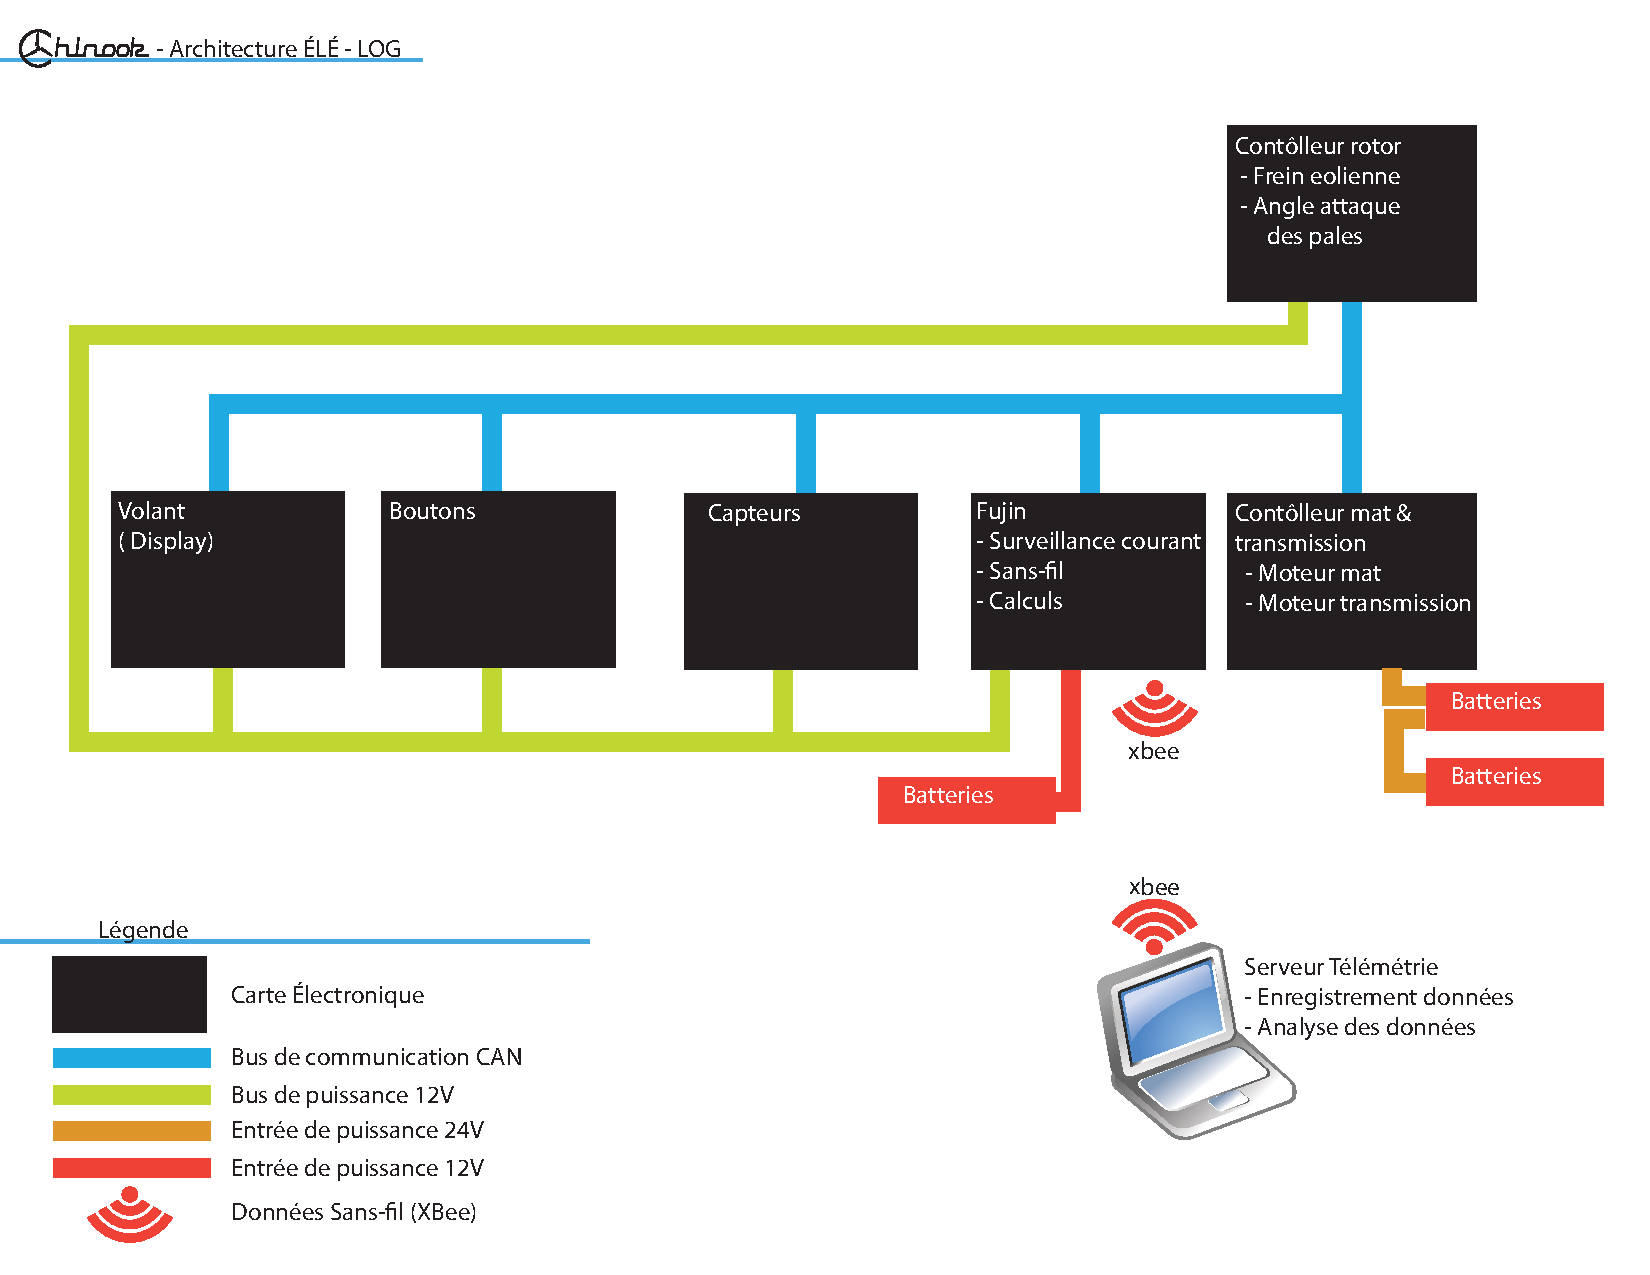
\includegraphics[height=1\textwidth,angle=90]{images/architecture-ele-log.pdf}

\clearpage
\section{Calcul de l'impact, la probabilité et de l'exposition aux risques}
\label{annexePERIL}
Voici les tableaux représentant le calcul de l'impact, la probabilité et l'exposition des risques selon la méthode de PERIL.

\subsection{Niveaux de probabilités/Impact}


\begin{tabu} to \linewidth {lX}
  \textbf{Terme} & \textbf{Définition} \\
  \hline
  Haut & Risque qui aurait une forte probabilité ou dont l'impact risquerait de mettre le bon bon déroulement du projet en jeu (retard de plusieurs jours) \\
  Moyen & Risque qui aurait une moyenne probabilité de survenir ou dont l'impact risquerait de retarder le projet de quelques jours.\\
  Bas & Risque qui aurait une faible probabilité de survenir ou dont l'impact risquerait de ne peu ou pas retarder le projet (quelques heures). 
\end{tabu}

\subsection{Calcul de Probabilité/Impact}

\begin{table}[H]
  \begin{center}
    \begin{tabu} to 0.5\linewidth {X[m]X[c,m]X[r,m]}
      \textbf{Niveau} & \textbf{Calcul} & \textbf{Probabilité ou Impact} \\
      \hline
      Haut  & \scalebox{1}{$\frac{1+ \frac{1}{2} +\frac{1}{3}}{3}$} & $0.6111$\\
      Moyen & $\frac{\frac{1}{2} +\frac{1}{3}}{3}$                  & $0.2777$\\
      Bas   & $\frac{\frac{1}{3}}{3}$                               & $0.1111$\\
    \end{tabu}
  \end{center}
\end{table}

\subsection{Exposition au risque}
L'exposition au risque est la probabilité multipliée par l'impact

\begin{table}[H]
  \begin{center}
    \begin{tabu} to 0.7\linewidth {X[1]|X[1]|X[1]|X[1]}
      & \textbf{Haut}     & \textbf{Moyen}    & \textbf{Bas} \\
      \hline
      Haut    & $0.3734$ & $0.1698$ & $0.0679$\\
      \hline
      Moyen   & $0.1698$ & $0.0712$ & $0.0309$\\
      \hline
      Bas     & $0.0679$ & $0.0309$ & $0.0123$\\
    \end{tabu}
  \end{center}
\end{table}
